\documentclass[a4paper]{article}
\usepackage[french]{babel}
\usepackage[utf8]{inputenc}
\usepackage{graphicx}

%%\usepackage{algorithm}
%%\usepackage{algorithmic}

%%%%%%%%%% marges %%%%%%%%%%

%%\usepackage{layout}
\usepackage[top=3cm, bottom=3cm, left=4cm, right=4cm]{geometry}



\begin{document}

\title{Manuel d'utilisation de Guitar tutor}

\maketitle

\tableofcontents{}
\newpage

\section{Description}
GuitarTutor est un projet permettant d'analyser avec un ordinateur un morceau joué à la guitare. Il est à vocation didactique, et à été réalisé par le Labri, 
puis repris par des élèves de l'ENSEIRB-MATMECA. Ce projet comprend à ce jour deux logiciels :
\begin{itemize}
\item  Le Player est un logiciel qui permet de comparer des accords joués à la guitare avec une représentation numérique d'un morceau de musique.
\item  L'Editeur est un logiciel qui permet d'enregistrer avec une interface graphique des morceaux de musique afin qu'ils soient utilisé par le Player.
\end{itemize}
Ce document  explique comment procéder pour utiliser toutes les fonctionnalités de vos deux logiciels \textbf{Editeur} et \textbf{Player} de GuitarTutor.
\newpage

\section{Installation}

\subsection{Compatibilité}
L’installation du Player et de l’Editeur sont possibles sous mac et sous linux.
\subsection{Description des délivrables}
Vous avez deux délivrables différents, l'un à destination des professeurs, l'autre à destination des élèves. 
Celui pour les professeurs contient à la fois le Player et l'Editeur, alors que celui pour les élèves ne contient que le Player.
\subsection{Procédure d'installation}
Pour installer le Player et/ou l'Editeur il vous suffit simplement de double cliquer sur le \textbf{setup} dans le répertoire correspondant à votre plateforme. 
Des boites de dialogues vont alors vous guider dans les étapes d'installation du logiciel. 
Vous allez notamment préciser le répertoire dans lequel vous voulez installer le logiciel, et autoriser l'installation de librairies supplémentaires.
L'installation peut être longue, cela est dû notemment à l'installation des librairies supplémentaires.
\subsection{En cas d'échec} 
Si l'installation du Player échoue, c'est qu'il y a certainement eu un problème dans l'installations des librairies supplémentaires, vous devez donc installer manuellement les librairies suivantes : \\
\underline{Sous linux}:
\begin{itemize}
\item Libqt4-dev
\item Portaudio19
\item Libsndfile1-dev
\end{itemize}
\underline{Sous mac}:
\begin{itemize}
\item Qt-4-base-mac'4.7.3-3
\item Portaudio 18.1-3
\item Libsndfile1-dev 1.0.25-1 
\end{itemize}
Si l'installation de l'éditeur échoue encore, il faut alors télécharger et installer la dernière librairie nécessaire : FMODEX. Vous devez installer manuellement la librairie suivantea : 
\begin{itemize}
\item Libfmodex4
\end{itemize}
Qui est téléchargeable ici: \begin{verbatim}
http://www.fmod.org/fmod-downloads.html
\end{verbatim} 
Aller à la partie concernant FMOD ex, puis télécharger la version stable correspondant à votre plateforme.
\newpage
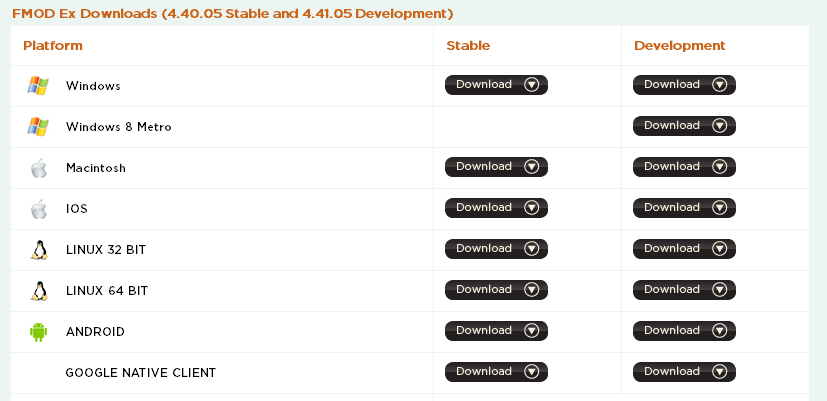
\includegraphics[scale=0.5]{manulutil1.png}
\newpage 
\section{Editeur}
L'éditeur comprend pour le moment :
\begin{itemize} 
\item Création d'un morceau ; vous serez invité à créer une grille et rentrer le rythme du morceau.
\end{itemize}
En le lançant vous aurez pourrez y accéder grâce au bouton :\\ 
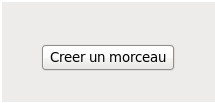
\includegraphics[scale=0.5]{manulutil2.png}
\subsection{Création d'un morceau}
\textbf{Les accords}\\
Pour commencer à numériser un morceau, vous devez rentrer les accords dans une grille d'accords. 
Vous avez la possibilité de faire varier le nombre de ligne et de colonne de cette grille. 
En plus des colonnes d'accords il y en a une d'annotation.
Le choix du nombre de colonnes se fait au moment de la création d'une nouvelle grille grâce au bouton \textit{new}.\\
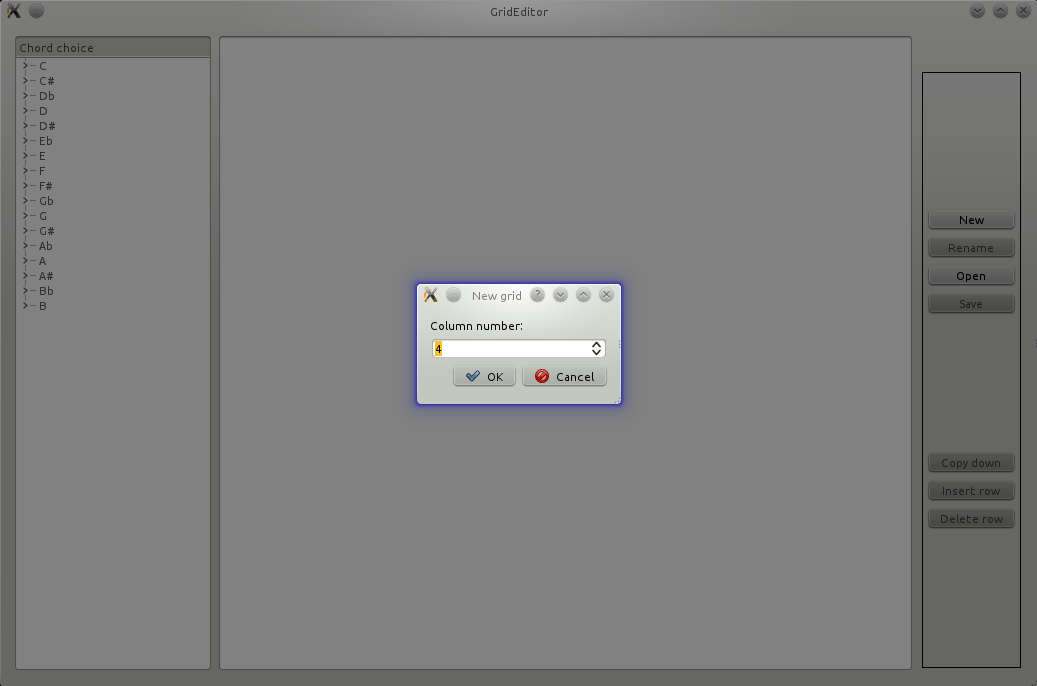
\includegraphics[scale=0.5]{manulutil3.png}\\
Le nombre de lignes, lui, peut être modifié à la volée en insérant des lignes à l'endroit souhaité.
Pour remplir les cases avec des notes, vous devez sélectionner une ou plusieurs cases, et choisir ensuite dans la liste hiérarchique de gauche l'accord que vous souhaitez en double cliquant dessus. 
En cliquant sur les fondamentales de la liste d'accords, les variantes vous sont affichées.\\
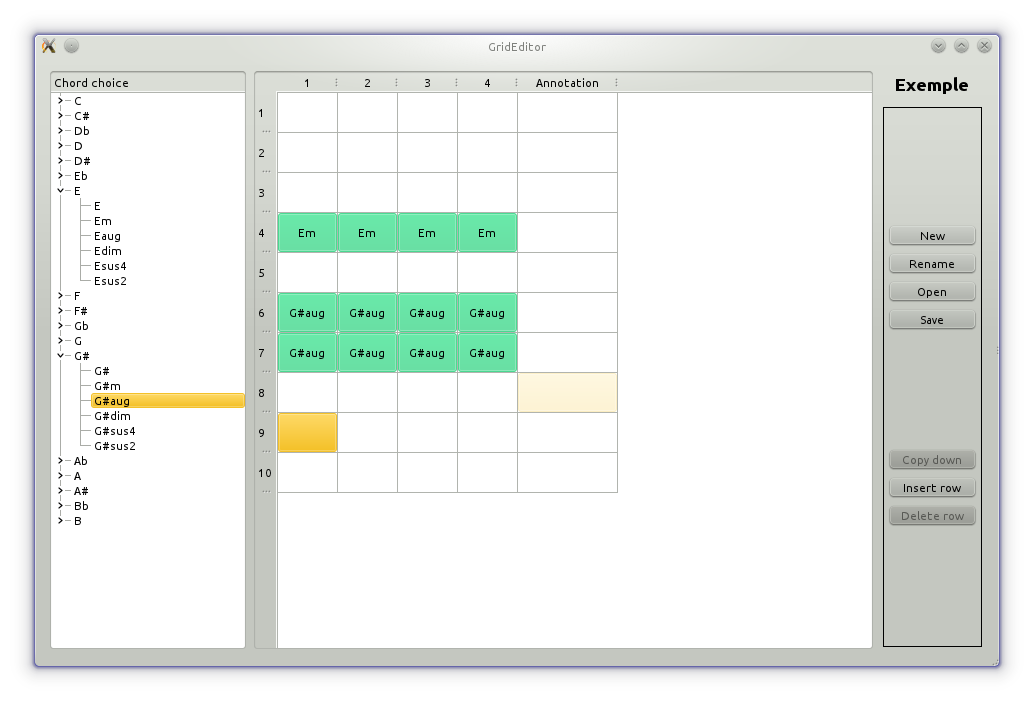
\includegraphics[scale=0.5]{manulutil4.png}\\
Vous pouvez supprimer une ou plusieurs lignes en les sélectionnant, puis en cliquant sur le bouton \textit{delete row} à droite.\\
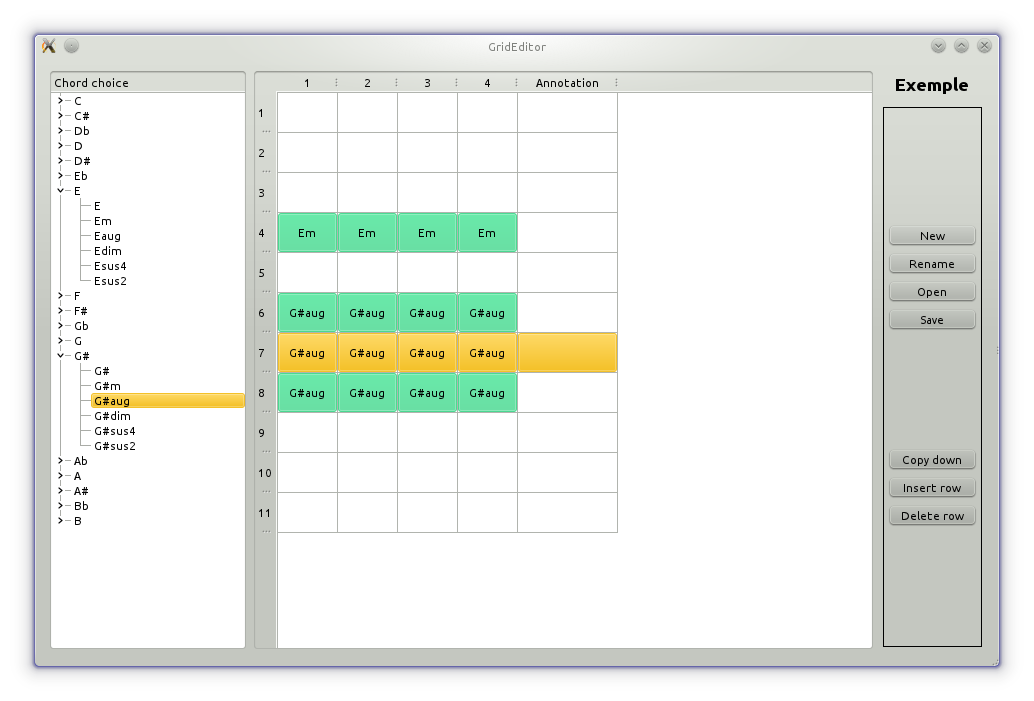
\includegraphics[scale=0.5]{manulutil5.png}\\
Les cases d'annotations sont des cases de texte libre. Vous pouvez renseigner les informations que vous voulez.\\
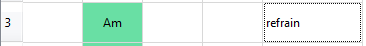
\includegraphics[scale=0.5]{manulutil6.png}\\
Il est possible de copier la ligne ou un bloc de ligne vers le bas. 
Il faut sélectionner le cloc souhaité et utiliser le bouton \textit{copy down}. 
Les nouvelles lignes sont insérées en dessous du bloc sans modifier le reste de la grille.\\
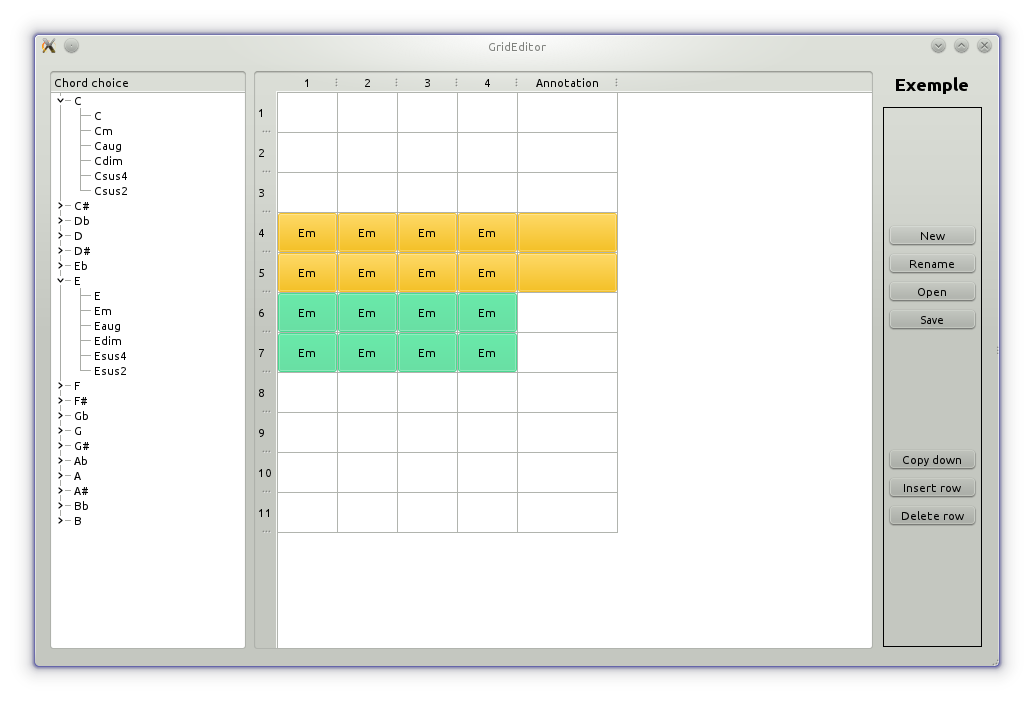
\includegraphics[scale=0.5]{manulutil7.png}\\
Le bouton \textit{Save} permet de sauvegarder la grille courante, terminée ou non, au format xgrid. 
La sauvegarde se fait dans le répertoire par défaut. 
Si la grille n'a pas encore été nommée, il faut lui en donner un avant la sauvegarde.
Le bouton \textit{Open} permet de choisir une grille au format xgrid et de l'ouvrir, elle peut ensuite être modifiée.
Vous pouvez continuer la numérisation du morceau avec la saisie des temps en appuyant sur le bouton \textit{continuer} en bas à droite.
\newpage 
\textbf{Le tempo}\\
Ensuite vous continuez avec la saisie du tempo. 
Vous devez choisir le fichier son au format .wav correspondant à la grille des accords préalablement créé. 
Pour cela aller dans l'onglet file puis \textit{ouvrir}, ou utiliser le bouton \textit{open} en bas de la fenêtre. 
Dans la nouvelle fenêtre qui s'ouvre vous pouvez naviguer dans vos répertoires et choisir le morceau.\\

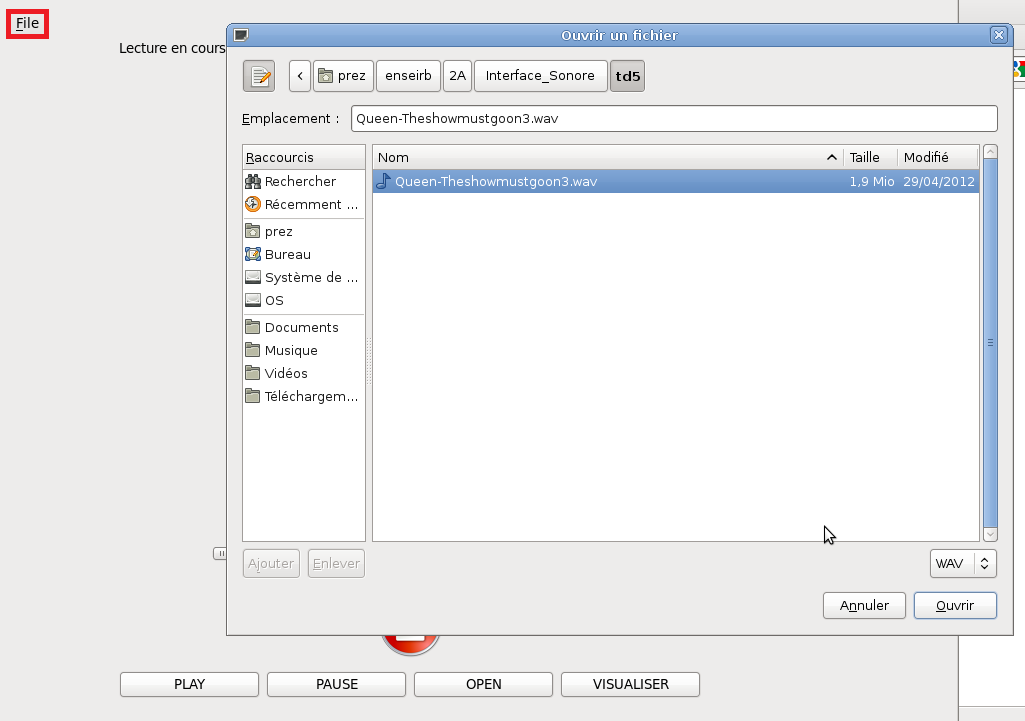
\includegraphics[scale=0.5]{manulutil8.png}\\
Une fois que vous avez choisi votre morceau, vous verrez la fenêtre suivante avec trois autres boutons : 
\begin{itemize}
\item  Play : ce bouton lance l'audio du morceau, et vous permet de saisir avec la barre espace le moment ou l'élève devra jouer l'accord qui est dans la grille défilante au dessus.
\item  Pause : permet de mettre le morceau en pause.
\item  Visualiser : permet de visualiser la saisie du tempo précédent. En cliquant sur ce bouton puis en faisant reculer le curseur, vous pourrez voir les moments ou vous avez appuyé sur la barre espace grâce au bouton rouge qui clignotera.\\
\end{itemize}
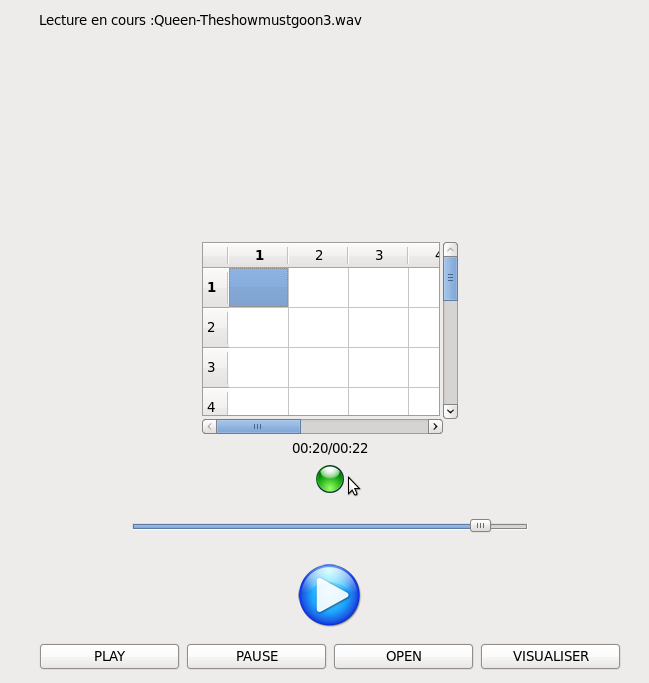
\includegraphics[scale=0.5]{manulutil9.png}\\
Le bouton vert passe au rouge à chaque fois que vous appuyez sur la barre espace, cependant dans le cas d'appuie répétitif trop rapide le bouton peut rester au rouge sans revenir au vert. 
L'enregistrement s'effectue dans tous les cas correctement. \\

Pour sauvegarder la saisie, aller dans l'onglet \textit{file} en haut de la fenêtre, puis cliquer sur \textit{exporter}. 
Le morceau est alors utilisable par le logiciel Player, pour être joué par un élève.
\subsection{Le curseur}  
Le curseur vous permet de vous déplacer dans le morceau, aussi bien dans l'écoute que dans la saisie des temps. 
Pour bouger le curseur il faut que vous le fassiez glisser, vers l'avant ou vers l'arrière.\\
Si vous êtes en train de saisir et que vous faites une erreur, vous pouvez donc revenir en arrière en déplaçant le curseur et vous corriger. 
Attention dès que vous faites glisser le curseur en arrière, les temps qui sont situés après la nouvelle position du curseur sont supprimés.\\
Si vous avez cliqué sur le bouton \textit{visualiser} vous pouvez revenir en arrière avec le curseur sans que cela supprime les temps.
\subsection{Raccourcis} 
Pour vous aider, et vous faire gagner du temps voici quelques raccourcis qui permettent d'obtenir les mêmes actions que les boutons : 
\begin{itemize}
\item  entrée : play/pause
\item  espace : saisir un temps
\item  \textit{ctrl + o} : ouvrir une musique \textit{.wav} 
\item  \textit{ctrl + e} : finir et exporter le fichier créé
\end{itemize}
\newpage 
\section {Player} 
La partie Player vous permet de sélectionner grâce à une liste déroulante le morceau que vous voulez jouer. 
Puis ensuite vous verrez les accords du morceau défiler sur la partie gauche.\\
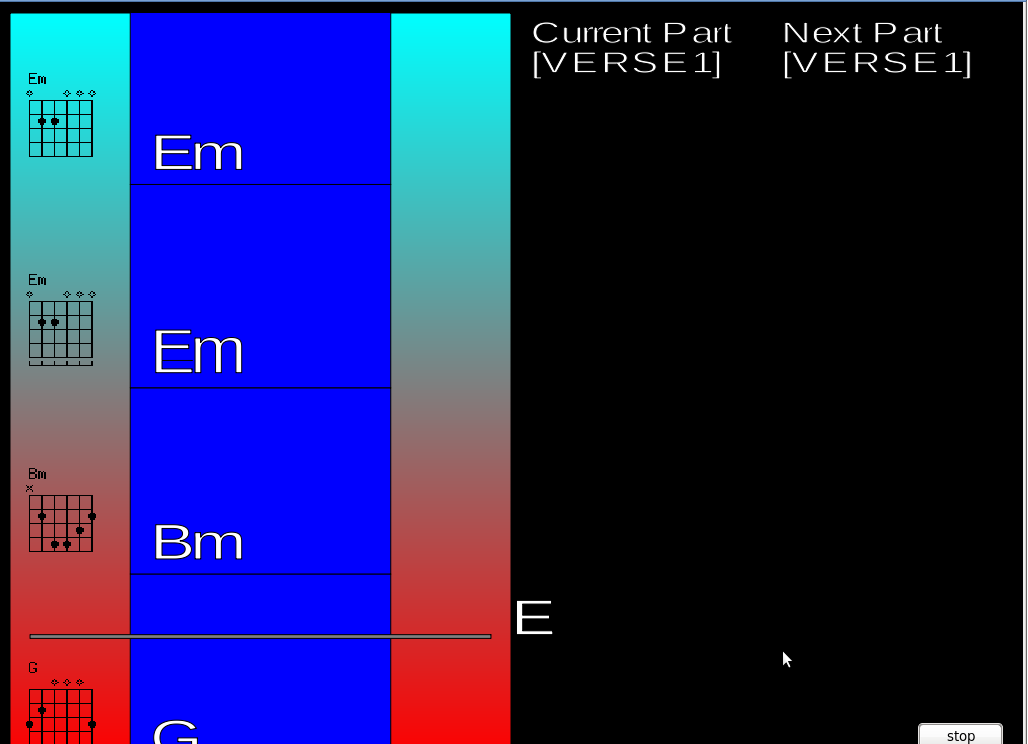
\includegraphics[scale=0.5]{manulutil10.png}\\








\end{document}
